% !TeX root = ../main.tex
% !TeX program = xelatex
% !TeX encoding = UTF-8
\section{多场景多尺度源荷协同优化方法}\label{minor:algorithm}

\subsection{多尺度变量与衔接}

模型由城市层、区域层和用户层构成。三个算例各取 3 个模型节点（2 个为聚合需求节点），乌鲁木齐、固原、武汉分别含 7、6、7 类热源与 3、2、1 条聚合管段。城市层确定机组新增与退役容量、温位模式、候选管径、储热规模与配电增容；区域层在 75/45~$^{\circ}$C 两级温位上建立逐时能量平衡，阻止低温热源直接供应高温需求；用户层按式(\ref{eq:agg-thermal})递推聚合节点的等效热状态，把负荷转移折算为节点需求的增减。三层通过容量、温位与建筑改造三类量衔接：用户侧负荷削减使节点需求下降，优先减少边际热源出力，恢复时由储热与可调热源响应。乌鲁木齐与武汉场景采用投资—运行联合 MILP；固原因问题规模采用锚定两阶段方法，先确定投资模式，再冻结投资开展全季运行校核，其推荐方案用于工程可行性比较。

\begin{figure}[H]
\centering
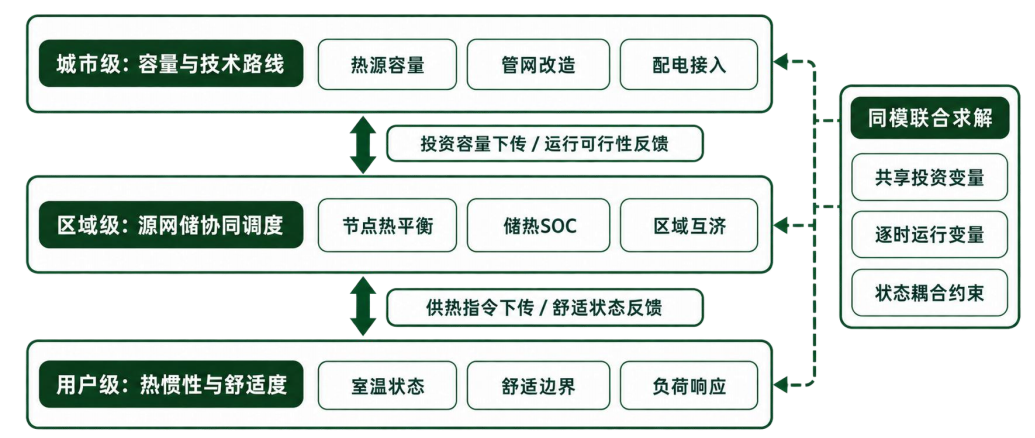
\includegraphics[width=0.60\textwidth,height=0.26\textheight,keepaspectratio]{media/algorithm-revision/fig2.png}
\caption{城市—区域—用户多尺度衔接}
\label{fig:alg-multiscale}
\end{figure}

\subsection{多目标协同优化}\label{minor:multiobjective}

成本与碳排放采用 $\varepsilon$-约束法协调\supcite{32}，模型以等年值净成本最小为目标并设置碳排放上限，逐档收紧后重解完整窗口，相邻两档的成本增量与减排量之比即边际减排成本。乌鲁木齐场景中，成本端点为 27.49 万元、27.32~t~CO$_2$，排放端点为 74.81 万元、10.57~t~CO$_2$；本文推荐记录采用通过该记录已启用硬约束与校核的方案，等年值成本为 27.76 万元、碳排放为 27.31~t~CO$_2$，与按目标函数排序得到的成本端点分开标注；候选点分布见附录5.8。零失供、清洁热比例与 $N-1$ 容量裕度按硬边界处理，边界内移峰由惩罚成本优化。

\begin{figure}[H]
\centering
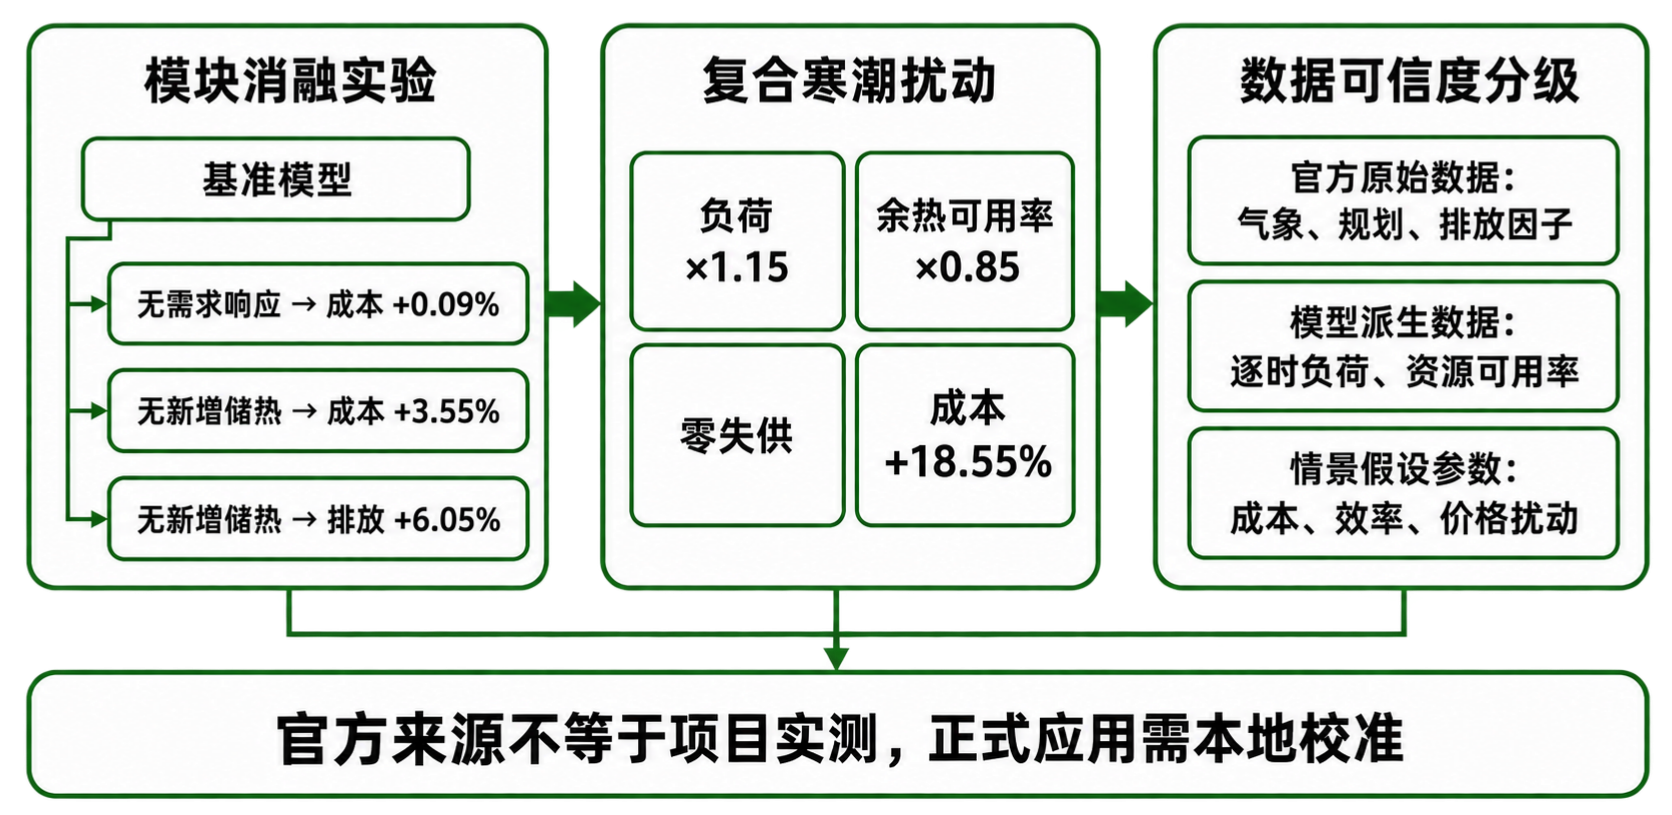
\includegraphics[width=0.60\textwidth,height=0.25\textheight,keepaspectratio]{media/algorithm-revision/fig5.png}
\caption{消融实验、扰动检验与数据可靠性}
\label{fig:alg-ablation}
\end{figure}

气象不确定性由独立风险层处理：

\begin{equation}
\min\ \mathbb{E}[C]+\lambda\operatorname{CVaR}_{\alpha}(C),
\qquad \alpha=0.8,
\label{eq:alg-risk-objective}
\end{equation}

其中 $\lambda$ 取 0、0.02、0.05、0.10 四档，条件风险价值按 Rockafellar--Uryasev 线性化：

\begin{equation}
\operatorname{CVaR}_{\alpha}(C)=\min_{\eta,z_s}\left\{\eta+\frac{1}{1-\alpha}\sum_s p_sz_s\right\},
\quad z_s\geq C_s-\eta,\quad z_s\geq0.
\label{eq:alg-cvar}
\end{equation}

$\lambda=0.05$ 为三个场景的统一参考值，风险层按独立记录登记。

\begin{figure}[H]
\centering
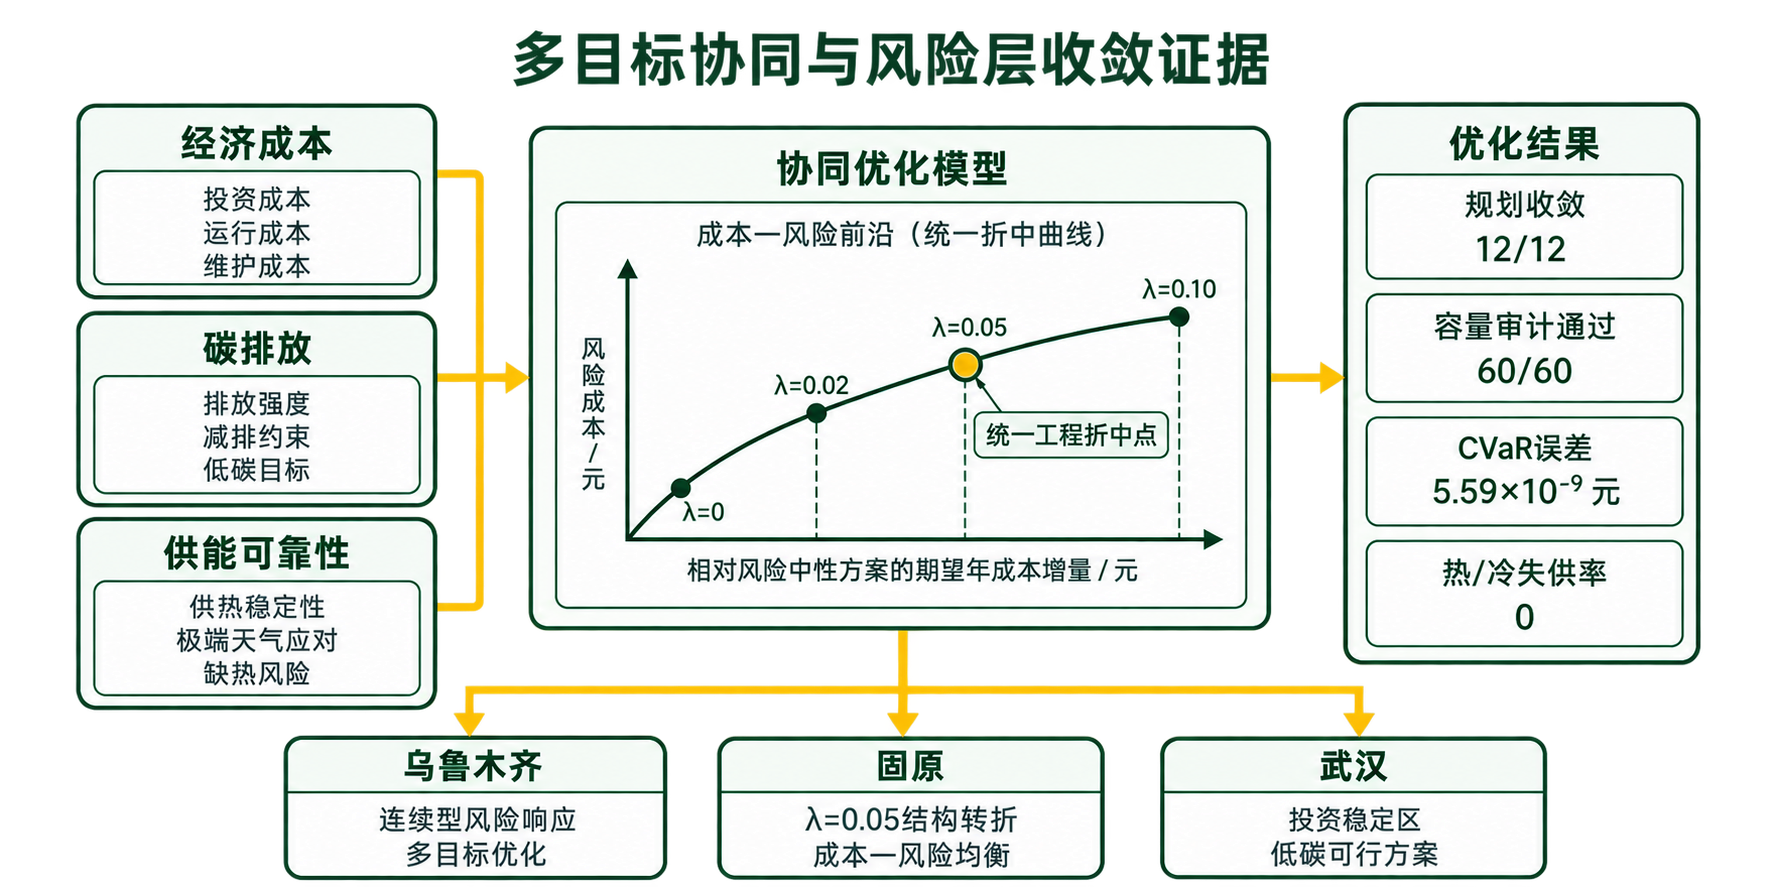
\includegraphics[width=0.60\textwidth,height=0.26\textheight,keepaspectratio]{media/algorithm-revision/fig3.png}
\caption{多目标协同与风险层收敛证据}
\label{fig:alg-objectives}
\end{figure}

\subsection{求解流程与收敛准则}

模型构造器采用 Python~3.11 实现，通过 SciPy 的 \texttt{milp} 调用 HiGHS 求解；约束按 CSR/CSC 稀疏格式编译和缓存，装配为完整模型约需 1.6~s，其中约束编译与缓存占 0.18~s。机组启停采用凸包重建模，开机状态保留为二元变量，辅助变量连续化。求解与复核顺序见算法\ref{alg:season-workflow}。

% !TeX root = ../main.tex
\newcounter{paperalgorithm}
\newenvironment{paperalgorithm}[2]{%
  \par\Needspace{12\baselineskip}\refstepcounter{paperalgorithm}\label{#2}%
  \begingroup\small\setstretch{1.05}\setlength{\parskip}{3pt}%
  \noindent\rule{\linewidth}{0.6pt}\par\noindent\textbf{算法\thepaperalgorithm\quad #1}\par
}{\par\noindent\rule{\linewidth}{0.6pt}\par\endgroup}

\begin{paperalgorithm}{窗口求解与逐时复核流程}{alg:season-workflow}
\noindent\textbf{输入：}场景配置、规划输入、连续窗口逐时数据与求解容差。\par
\noindent\textbf{输出：}投资及逐时运行方案，求解状态、间隙与校核记录。
\begin{enumerate}[label=\arabic*.,leftmargin=1.8em,itemsep=2pt,topsep=3pt,parsep=0pt]
\item 核对窗口、步长、单位与各模块启用状态。
\item 按第2章约束装配源网荷储电模型，联立守恒、容量与热状态条件并设初末边界。
\item 乌鲁木齐联合求解投资与运行；固原、武汉冻结投资模式后求解全季运行。
\item 按碳帽或 $\varepsilon$ 档位重复求解并逐档保存。
\item 记录目标值、上下界、间隙、时间与可行性状态。
\item 以逐时输出复算守恒、状态、容量、资源与失供核对。
\item 导出可核结果并标注求解身份与逐时调度。
\end{enumerate}
\end{paperalgorithm}


优化器一次求解整个声明窗口，求解状态、间隙、残差与后验校核分别登记，时限内可行解保留近似解身份。乌鲁木齐联合模型的相对间隙为 $1.53\times10^{-4}$（531.1~s，启停二元 8784 个），武汉联合模型为 $3.27\times10^{-3}$（1960.5~s，整数变量 8642 个），固原运行层为 $1.84\times10^{-3}$（64.0~s，二元 4392 个）；各层间隙按求解身份分别登记。

\begin{figure}[H]
\centering
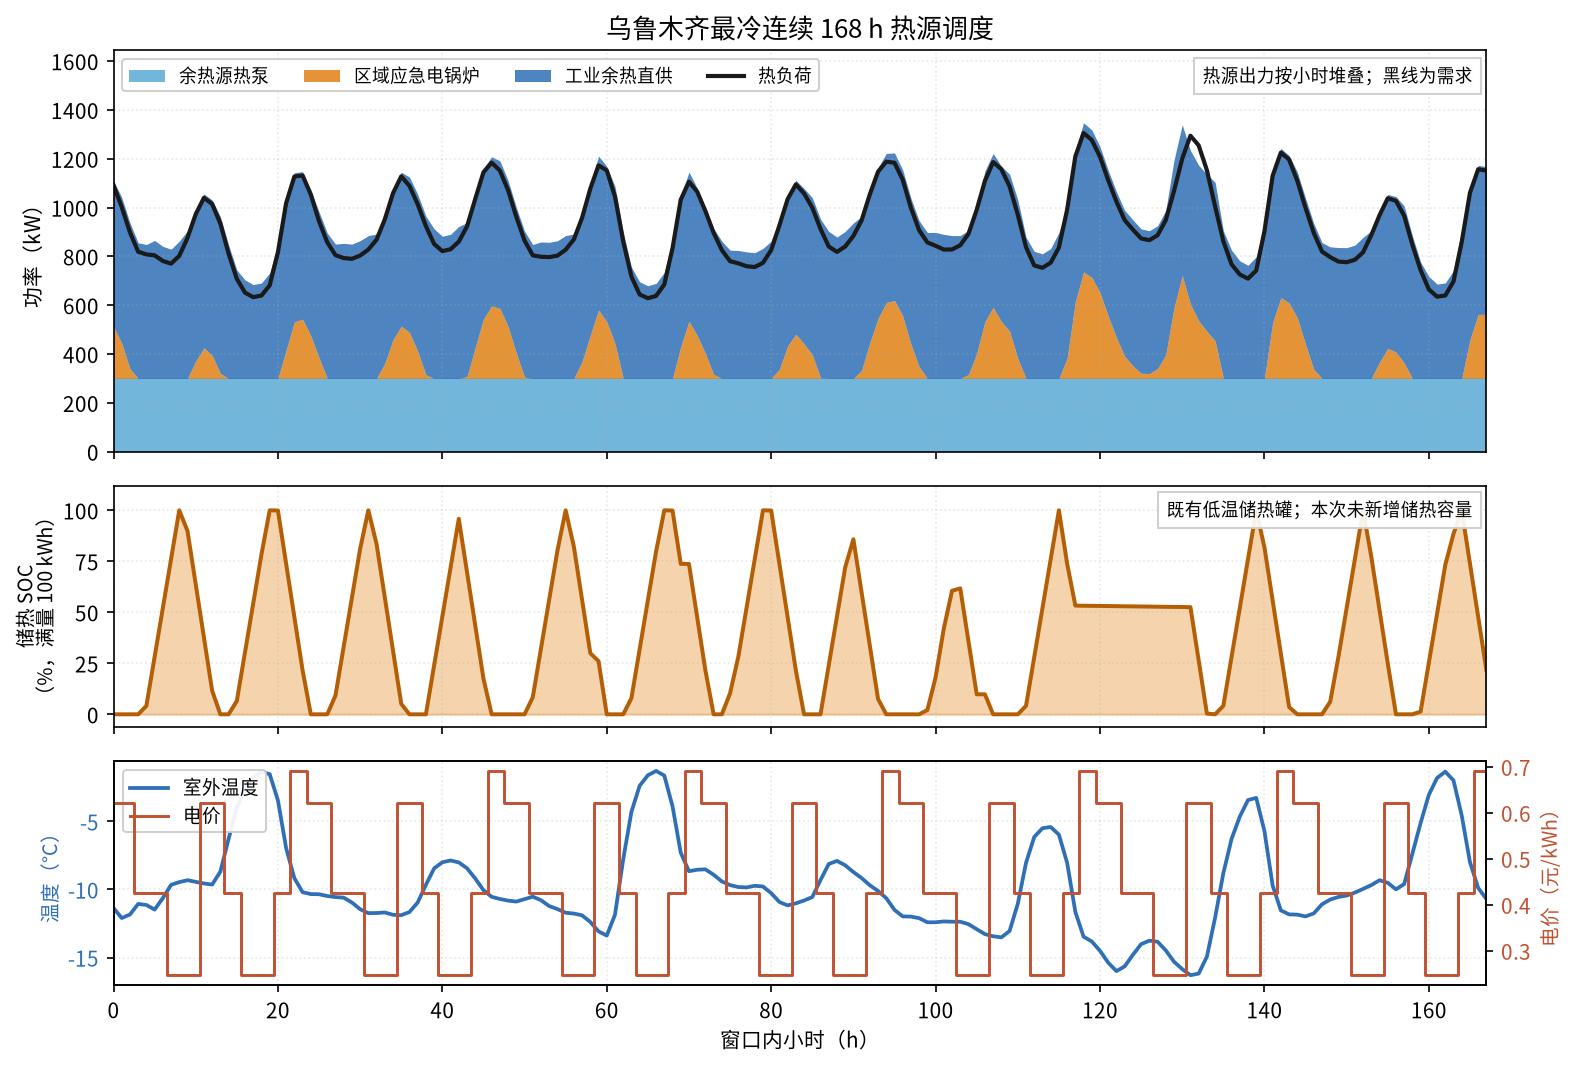
\includegraphics[width=0.78\linewidth,height=0.30\textheight,keepaspectratio]{media/r18/fig_coldest168.png}
\caption{乌鲁木齐最冷连续 168~h 热源调度与储热状态}
\label{fig:code-cold168}
\end{figure}

\subsection{计算效率与扩展性}

效率改善来自启停凸包重建模和稀疏编译缓存：固原两年度回放合计由 602.483~s 降至 112.750~s，减少 81.29\%，整数变量由 26280 个减至 8760 个；单次窗口约含 31 万---45 万个变量。

\begin{figure}[H]
\centering
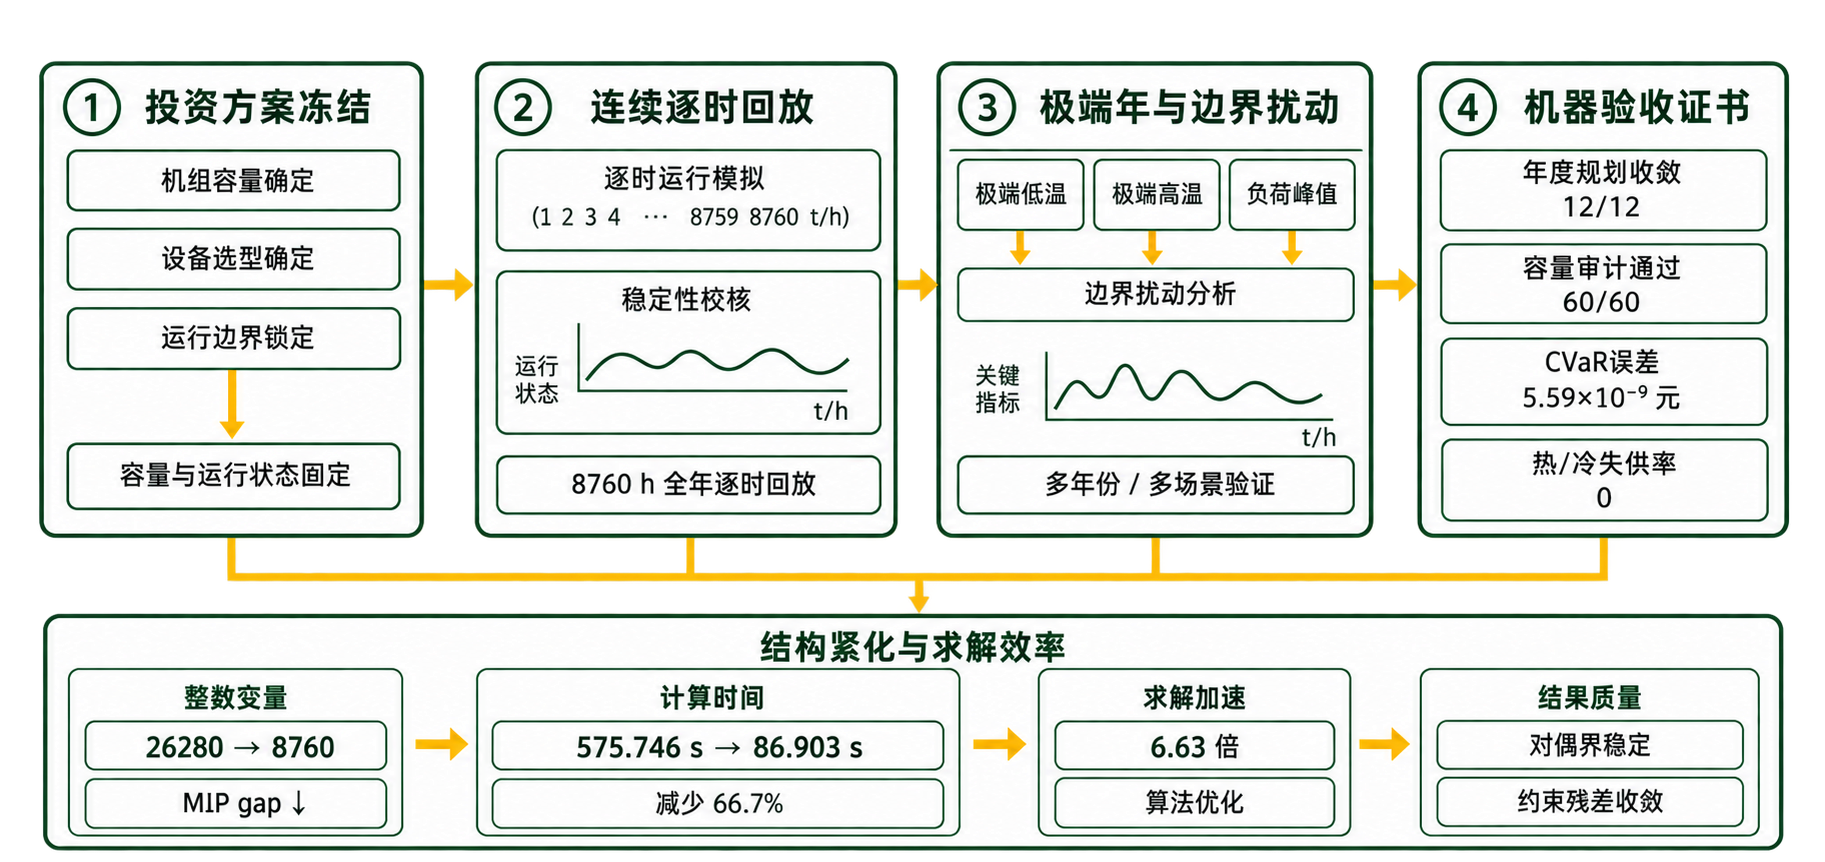
\includegraphics[width=0.60\textwidth,height=0.25\textheight,keepaspectratio]{media/algorithm-revision/fig4.png}
\caption{逐时回放、边界稳定性与求解效率}
\label{fig:alg-replay}
\end{figure}
